\section{Tiền xử lý dữ liệu}
\subsection{Tổng quan về dữ liệu}

\hspace{10pt}
File dữ liệu đầu vào được nhóm quyết định chọn trên nền tảng Kaggle có tên \textbf{Housing.csv} tại 
\href{https://www.kaggle.com/datasets/yasserh/housing-prices-dataset}{housing-prices-dataset}. Bộ dữ liệu gồm các thông tin như giá bất động sản, diện tích, số phòng ngủ, số phòng tắm, v.v. Mục tiêu của bài tập lớn này là tìm ra mối quan hệ giữa giá bất động sản và các đặc tính của căn nhà.\\
\hspace{10pt}

Bộ dữ liệu bao gồm 545 mẫu, mỗi mẫu đại diện cho một căn nhà với các cột đặc tính sau:
\begin{itemize}
	\item \textbf{price}: giá bán của căn nhà (đơn vị: USD)
	\item area: diện tích của căn nhà (feet vuông)
	\item bedrooms: số lượng phòng ngủ
	\item bathrooms: số lượng phòng tắm
	\item mainroad: có nằm ở mặt tiền hay không
	\item guestroom: có phòng khách hay không
	\item basement: có tầng hầm hay không
	\item hotwaterheating: có máy nước nóng hay không
	\item airconditioning: có điều hòa hay không
	\item parking: số lượng bãi đậu xe
	\item prefarea: thuộc khu vực ưu tiên hay không
	\item furnishingstatus: tình trạng nội thất (unfurnished, semi-furnished, furnished)
\end{itemize}

\subsection{Xử lý dữ liệu}

\subsubsection{Đọc dữ liệu}

\hspace{10pt}
Sau khi đọc dữ liệu, ta lưu vào Pandas DataFrame.\\
\hspace{10pt}

Hình bên dưới minh họa 5 dòng đầu trong bộ dữ liệu để có cái nhìn tổng quát hơn.
\begin{figure}[h]
	\centering
	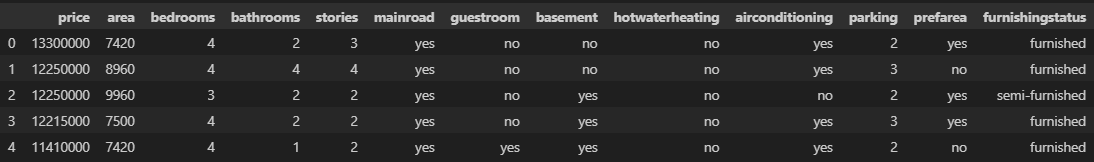
\includegraphics[width=\textwidth]{chapters/Preprocessing/images/demo_data.png}
	\caption{Thông tin cơ bản về tập dữ liệu}
\end{figure}

\subsubsection{Kiểm tra và xử lý dữ liệu khuyết}
\hspace{10pt}
Để kiểm tra dữ liệu khuyết và dữ liệu trùng trong tập dữ liệu, ta sử dụng 2 lệnh: 
data.isnull().sum() và data.duplicated().sum() để thống kê lại tổng số dữ liệu khuyết và dữ liệu trùng lặp trên từng cột:
\begin{figure}[h]
	\centering
	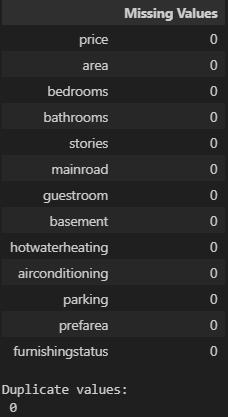
\includegraphics[width=0.3\textwidth]{chapters/Preprocessing/images/miss_value.png}
	\caption{Thống kê dữ liệu khuyết và trùng lặp}
\end{figure}

Dựa vào hình trên, ta có thể thấy rằng không có giá trị khuyết và giá trị trùng lặp tồn tại trong tập dữ liệu. Do đó, không cần xử lý dữ liệu khuyết cũng như dữ liệu trùng lặp.

\subsubsection{Xử lý dữ liệu phân loại}
\hspace{10pt}
Để kiểm tra sự tồn tại của dữ liệu phân loại trong tập dữ liệu, ta sử dụng lệnh \texttt{data.dtypes} nhằm thống kê các kiểu dữ liệu của các đặc trưng.

\begin{figure}[H]
	\centering
	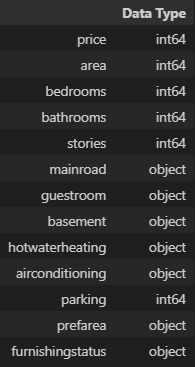
\includegraphics[width=0.3\textwidth]{chapters/Preprocessing/images/initial_dtype.png}
	\caption{Thống kê kiểu dữ liệu}
\end{figure}
\hspace{10pt}

Dựa vào hình, ta có thể thấy rằng các cột có kiểu dữ liệu là \texttt{object} gồm: \texttt{mainroad}, \texttt{guestroom}, \texttt{basement}, \texttt{hotwaterheating}, \texttt{airconditioning}, \texttt{prefarea}, và \texttt{furnishingstatus} -- đây là các cột chứa giá trị phân loại. Ta áp dụng kỹ thuật One-Hot Encoding để chuyển đổi các cột này thành các giá trị nhị phân tương ứng với từng loại giá trị. Ngoài ra, ta sẽ sử dụng tham số \texttt{drop\_first=True} để tránh trường hợp đa cộng tuyến. Sau khi xử lý, tập dữ liệu sẽ được chuyển hóa thành như sau:
\begin{figure}[H]
	\centering
	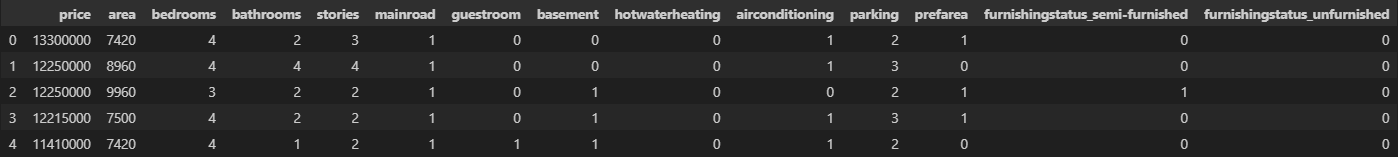
\includegraphics[width=\textwidth]{chapters/Preprocessing/images/dtype.png}
	\caption{Thống kê kiểu dữ liệu sau khi phân loại}
\end{figure}
\section{Phân tích dữ liệu}
\begin{figure}[H]
	\centering
	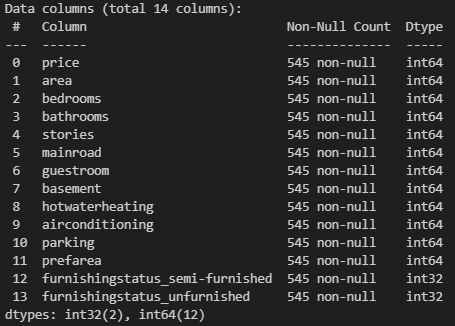
\includegraphics[width=0.7\textwidth]{chapters/Preprocessing/images/info_data.png}
	\caption{Tập dữ liệu sau khi xử lý}
\end{figure}
\hspace{10pt}

Trước khi phân tích dữ liệu, ta phân tích tổng quan dữ liệu sau tiền xử lý. Ta sử dụng \texttt{df.info()}. Dựa vào Hình 3.1, ta có thể rút ra được rằng:

\begin{itemize}
	\item Dữ liệu bao gồm 545 mẫu.
	\item Ở mỗi cột dữ liệu đều đếm được 545 dòng dữ liệu không rỗng.
	\item Tất cả 14 cột đều có kiểu \texttt{int64}.
\end{itemize}

Trong đó, biến dữ liệu được chia thành hai loại: biến liên tục và biến rời rạc.

\begin{itemize}
	\item Biến liên tục: là biến có thể nhận vô số giá trị $\rightarrow$ \texttt{area}.
	
	\item Biến rời rạc: là biến chỉ có thể nhận hữu hạn các giá trị riêng biệt $\rightarrow$ 
	\texttt{bedrooms}, \texttt{bathrooms}, \texttt{stories}, \texttt{parking}, 
	\texttt{mainroad\_yes}, \texttt{guestroom\_yes}, \texttt{basement\_yes}, 
	\texttt{hotwaterheating\_yes}, \texttt{airconditioning\_yes}, \texttt{prefarea\_yes}, 
	\texttt{furnishingstatus\_semi-furnished}, và 
	\texttt{furnishingstatus\_unfurnished}.
\end{itemize}

\section{Kiểm tra phân bố và outliers của "price"}

\hspace{10pt}
Trước khi phân tích sự tương quan của các thuộc tính, ta cần kiểm tra sự phân bố của
"price":
\begin{figure}[H]
	\centering
	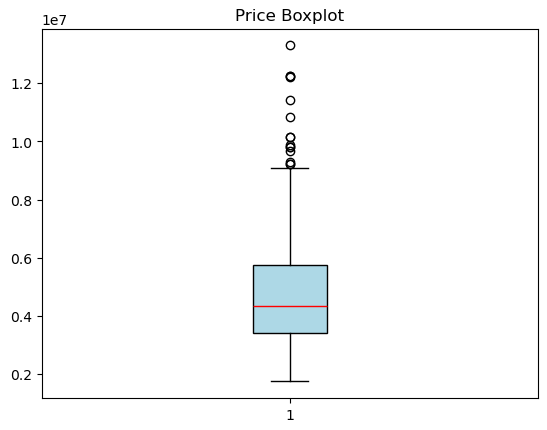
\includegraphics[width=0.7\textwidth]{chapters/Preprocessing/images/price_ouliers.png}
	\caption{Giá trị outliers của "price"}
\end{figure}
\begin{figure}[H]
	\centering
	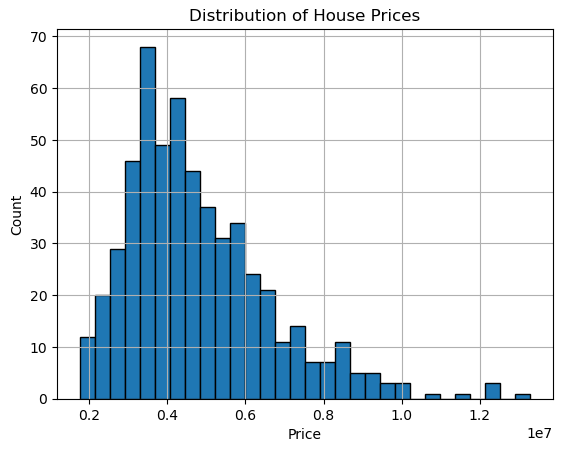
\includegraphics[width=0.7\textwidth]{chapters/Preprocessing/images/distribution.png}
	\caption{Biểu đồ phân bố "price"}
\end{figure}
\textbf{Đánh giá chung:} Biến \texttt{price} có phân phối lệch phải (right-skewed) rõ rệt, với phần lớn dữ liệu tập trung ở phân khúc giá thấp và trung bình (khoảng $3 \times 10^6$ đến $6 \times 10^6$). Cả hai biểu đồ đều xác nhận sự hiện diện của nhiều giá trị ngoại lệ (outliers) phía cao, cho thấy thị trường tồn tại một số bất động sản có giá trị đột biến so với mặt bằng chung. Đặc điểm này gợi ý rằng việc áp dụng biến đổi logarit có thể cần thiết để đưa dữ liệu về phân phối chuẩn hơn trước khi đưa vào các mô hình dự báo.
\subsection{Ma trận tương quan của các biến}

Để phân tích mối quan hệ giữa các đặc trưng trong tập dữ liệu, ta sử dụng ma trận tương quan. Ma trận này biểu diễn mức độ tương quan tuyến tính giữa các cặp thuộc tính, với giá trị nằm trong khoảng từ $-1$ đến $1$. Trong đó:

\begin{itemize}
	\item Giá trị gần $1$ biểu thị mối tương quan thuận mạnh.
	\item Giá trị gần $-1$ biểu thị mối tương quan nghịch mạnh.
	\item Giá trị gần $0$ biểu thị mối tương quan yếu hoặc không tồn tại.
\end{itemize}
\begin{figure}[H]
	\centering
	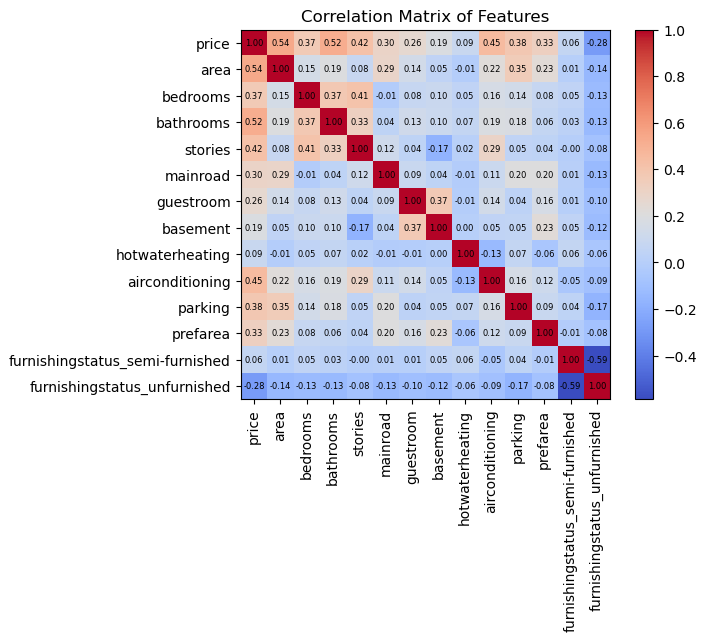
\includegraphics[width=0.9\textwidth]{chapters/Preprocessing/images/correlation.png}
	\caption{Biểu đồ tương quan giữa các biến}
\end{figure}
\hspace{10pt}

Dựa vào hình, ta nhận thấy một số biến có mối tương quan đáng kể với biến mục tiêu \texttt{price}. Cụ thể, các biến như \texttt{area} ($r = 0.54$), \texttt{bathrooms} ($r = 0.52$), \texttt{stories} ($r = 0.45$), và \texttt{airconditioning} ($r = 0.42$) có mức tương quan khá mạnh, cho thấy chúng có ảnh hưởng rõ rệt đến giá nhà. 

Bên cạnh đó, các biến như \texttt{bedrooms}, \texttt{parking}, \texttt{mainroad} và \texttt{prefarea} có hệ số tương quan ở mức trung bình ($0.30 \leq r < 0.4$), vẫn có thể được xem xét trong quá trình xây dựng mô hình.

Ngược lại, các đặc trưng như \texttt{basement}, \texttt{guestroom}, \texttt{hotwaterheating} và \texttt{furnishingstatus} có tương quan yếu hoặc gần như không có tương quan với giá nhà ($r < 0.2$), thậm chí có một số biến như \texttt{mainroad\_no} thể hiện mối quan hệ ngược chiều ($r = -0.28$).

\subsection{Trực quan hóa dữ liệu}

Trực quan hóa dữ liệu sẽ giúp ta hiểu rõ hơn về phân bố, xu hướng và mối quan hệ giữa các biến và biến \texttt{price}.

\begin{itemize}
	\item Biến liên tục: ta sử dụng boxplot để biểu thị sự phân bố của nó và scatterplot để
\end{itemize}
biểu hiện phân bố theo \texttt{price}

\begin{itemize}
	\item Biến rời rạc: ta sử dụng barplot để biểu thị sự phân bố của nó và boxplot để biểu hiện phân bố theo \texttt{price}
\end{itemize}

\subsubsection{Biến \texttt{area}}
\begin{figure}[H]
	\centering
	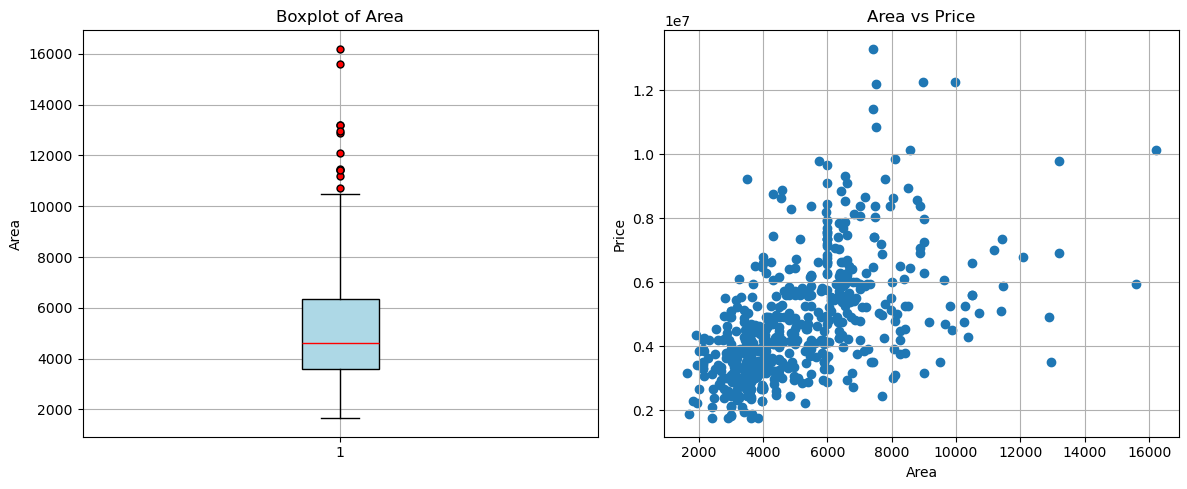
\includegraphics[width=\textwidth]{chapters/Preprocessing/images/area.png}
	\caption{Biến "area"}
\end{figure}

\subsubsection{Biến "bedrooms"}
\begin{figure}[H]
	\centering
	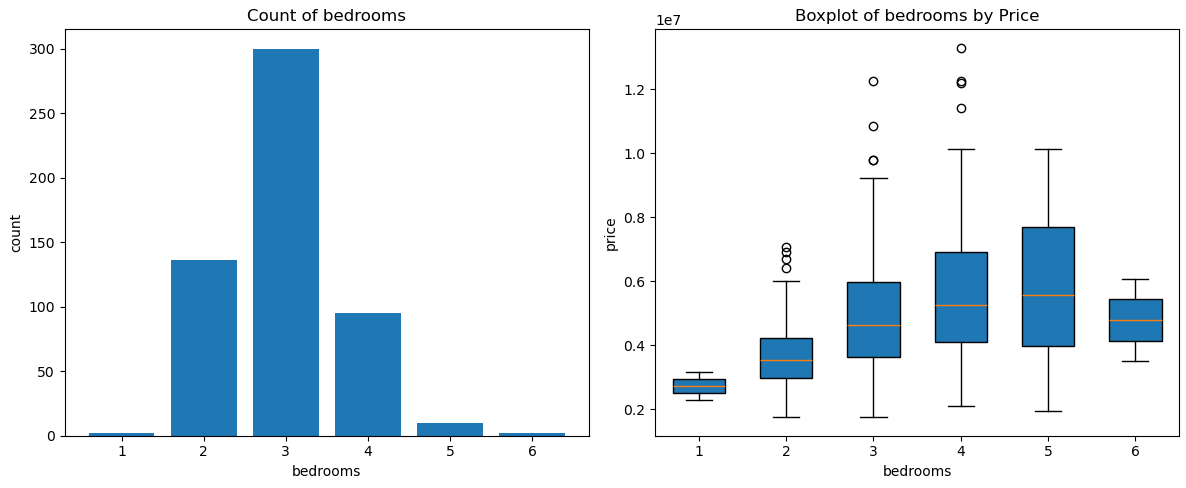
\includegraphics[width=\textwidth]{chapters/Preprocessing/images/bedroom.png}
	\caption{Biến "bedrooms"}
\end{figure}

\subsubsection{Biến "bathrooms"}
\begin{figure}[H]
	\centering
	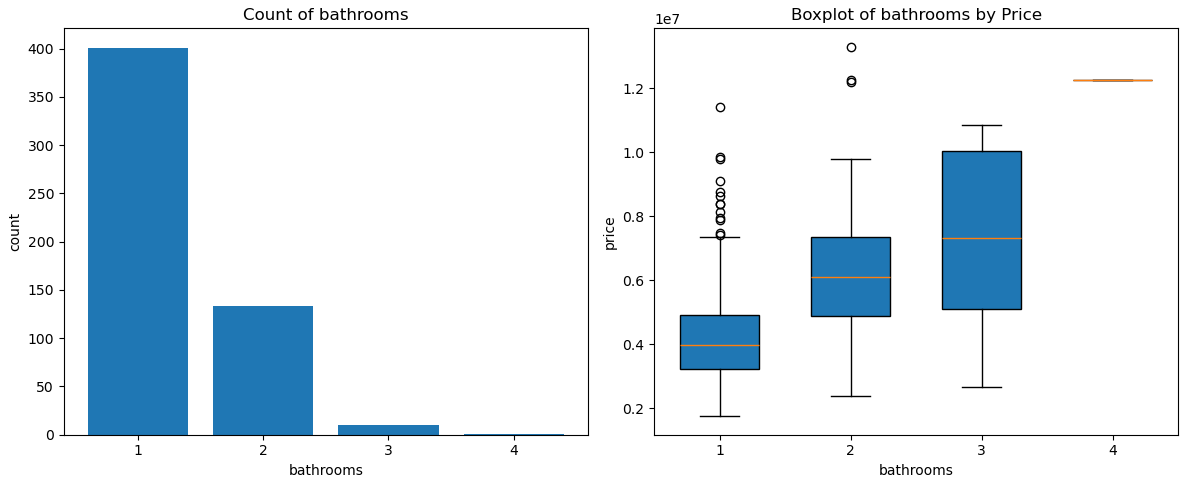
\includegraphics[width=\textwidth]{chapters/Preprocessing/images/bathroom.png}
	\caption{Biến "bathrooms"}
\end{figure}

\subsubsection{Biến "stories"}
\begin{figure}[H]
	\centering
	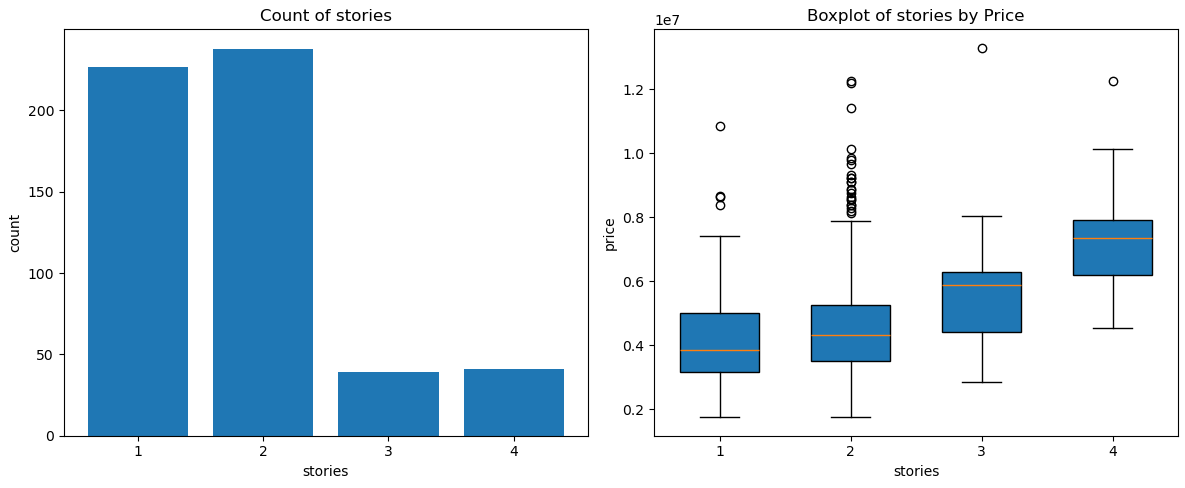
\includegraphics[width=\textwidth]{chapters/Preprocessing/images/storie.png}
	\caption{Biến "stories"}
\end{figure}

\subsubsection{Biến "parking"}
\begin{figure}[H]
	\centering
	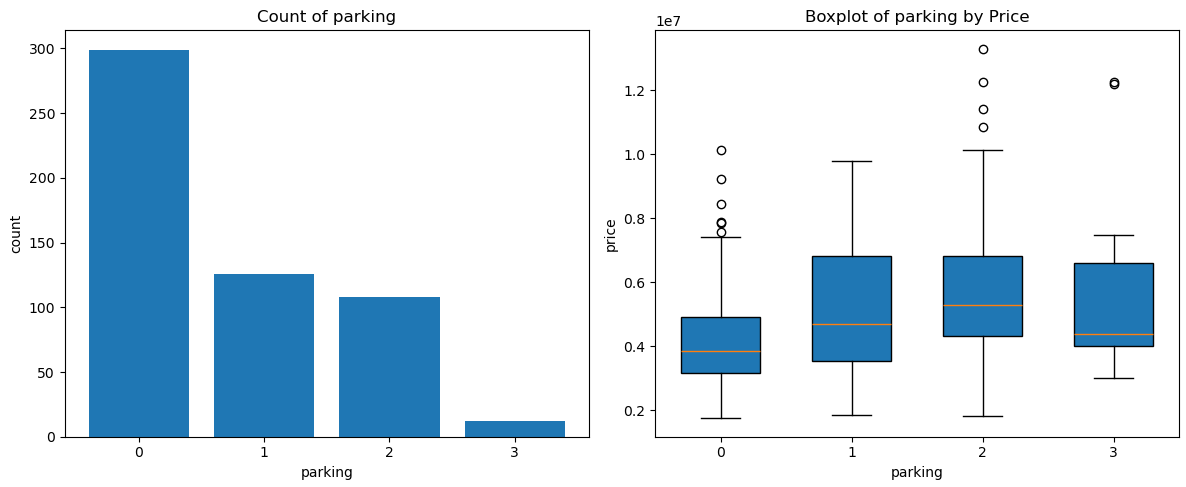
\includegraphics[width=\textwidth]{chapters/Preprocessing/images/parking.png}
	\caption{Biến "parking"}
\end{figure}

\subsubsection{Biến "mainroad"}
\begin{figure}[H]
	\centering
	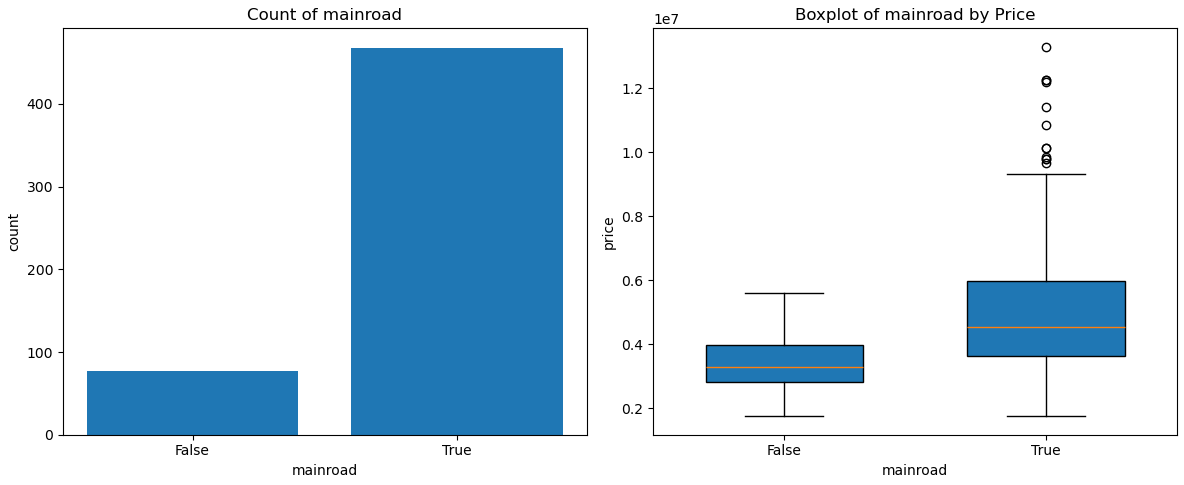
\includegraphics[width=\textwidth]{chapters/Preprocessing/images/mainroad.png}
	\caption{Biến "mainroad"}
\end{figure}

\subsubsection{Biến "guestroom"}
\begin{figure}[H]
	\centering
	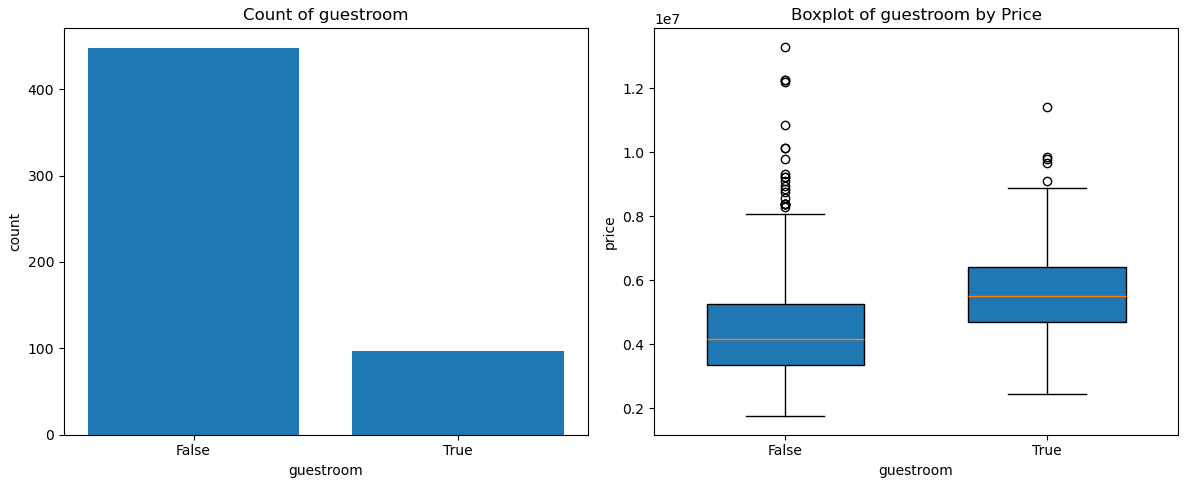
\includegraphics[width=\textwidth]{chapters/Preprocessing/images/guestroom.png}
	\caption{Biến "guestroom"}
\end{figure}

\subsubsection{Biến "basement"}
\begin{figure}[H]
	\centering
	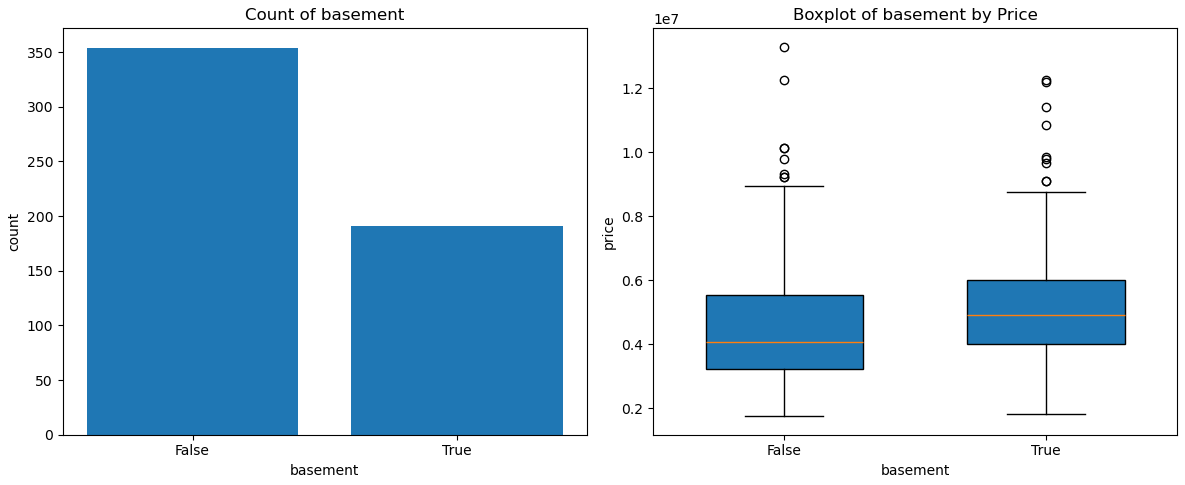
\includegraphics[width=\textwidth]{chapters/Preprocessing/images/basement.png}
	\caption{Biến "basement"}
\end{figure}

\subsubsection{Biến "hotwaterheating"}
\begin{figure}[H]
	\centering
	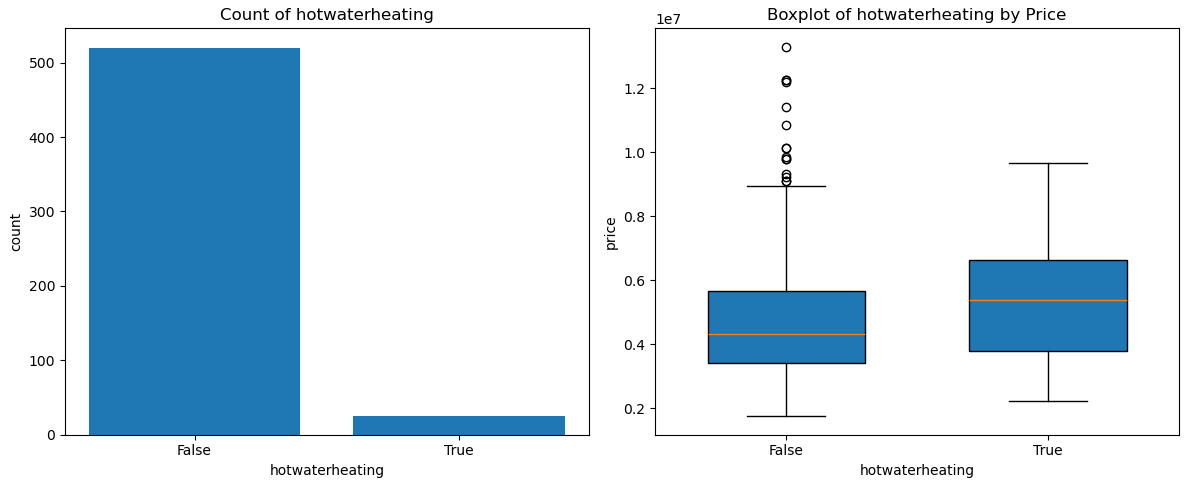
\includegraphics[width=\textwidth]{chapters/Preprocessing/images/hotwaterheating.png}
	\caption{Biến "hotwaterheating"}
\end{figure}

\subsubsection{Biến "airconditioning"}
\begin{figure}[H]
	\centering
	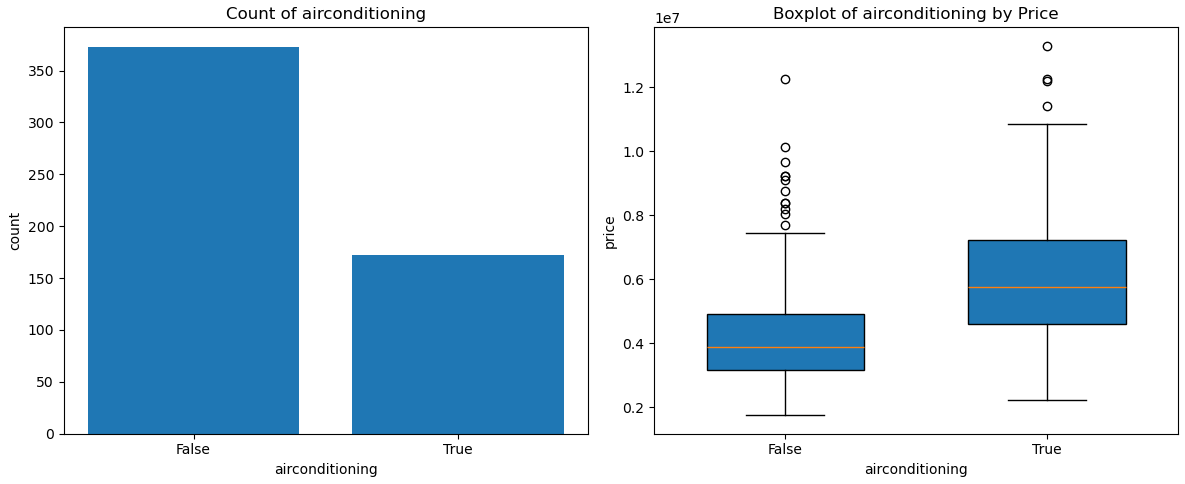
\includegraphics[width=\textwidth]{chapters/Preprocessing/images/airconditioning.png}
	\caption{Biến "airconditioning"}
\end{figure}

\subsubsection{Biến "prefarea"}
\begin{figure}[H]
	\centering
	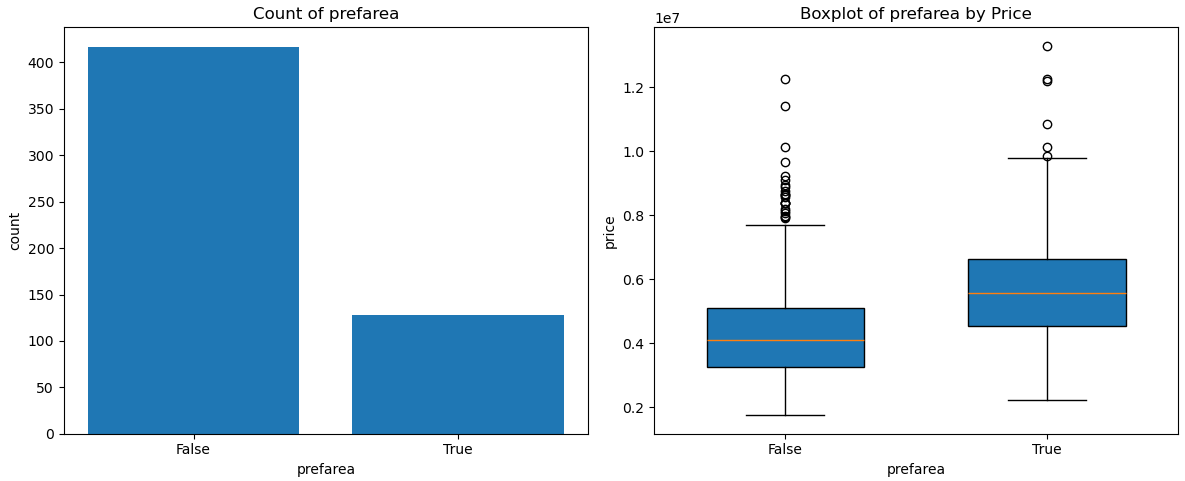
\includegraphics[width=\textwidth]{chapters/Preprocessing/images/prefarea.png}
	\caption{Biến "prefarea"}
\end{figure}

\subsubsection{Biến "furnishingstatus\_semi-furnished"}
\begin{figure}[H]
	\centering
	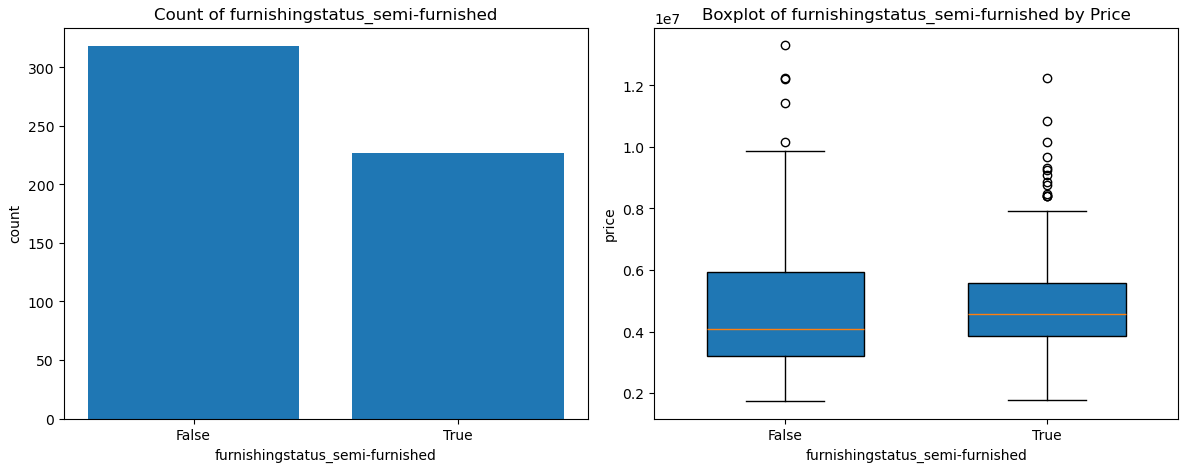
\includegraphics[width=\textwidth]{chapters/Preprocessing/images/semi-fur.png}
	\caption{Biến "furnishingstatus\_semi-furnished"}
\end{figure}

\subsubsection{Biến "furnishingstatus\_unfurnished"}
\begin{figure}[H]
	\centering
	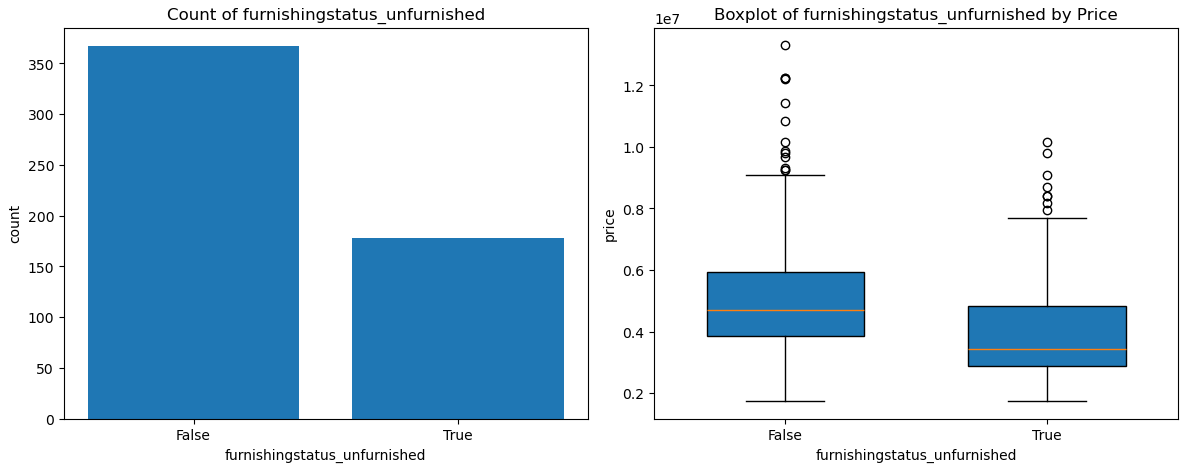
\includegraphics[width=\textwidth]{chapters/Preprocessing/images/unfur.png}
	\caption{Biến "furnishingstatus\_unfurnished"}
\end{figure}